\subsection{Отладка операций в функциональном стиле}
После появления функций высшего порядка и расширения стандартной библиотеки возможности JPDA остались прежними. Таким образом, с одной стороны, имеется способ записывать операции над множествами объектов в новом синтаксисе, с другой стороны, возможности отладчика остались прежними. Рассмотрим возможности отладчиков трех крупнейших сред разработки (Eclipse, NetBeans, IntelliJ IDEA), которые могут быть полезны при отладке цепочек методов, оперирующих потоком объектов.

\begin{itemize}
	\item Использование точек останова (с условием). Допускается, что точка останова будет внутри тела анонимной функции.
	\item Последовательные переходы по вызовам анонимных функций внутри цепочки.
	\item Вычисление выражений с анонимными функциями (доступно только в IDEA).
\end{itemize}

\subsubsection{Недостатки имеющихся подходов}
Описанные методы обладают недостатками, их не всегда удобно использовать и не всегда достаточно, чтобы понять причину ошибок.

Перечислим недостатки этих подходов.
\begin{itemize}
	\item При использовании точек останова внутри анонимной функции у нас есть только информация о текущем вызове и объект, при этом нельзя понять почему именно этот объект появился в данном месте, и какие трансформации он претерпел. Логичное предположение, что эту информацию можно восстановить в одном из элементов стека вызовов окажется неверным. Стек вызовов состоит из большого числа внутренних вызовов и нет гарантий, что получится там найти что-то полезное. Ниже приведен пример стека для достаточно простого вызова.
	\inputminted{java}{chapter1/code/SimplestStreamExample.java}
	
	И стек вызовов в точке останова внутри анонимной функции.
	
	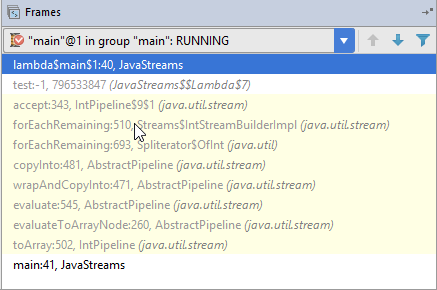
\includegraphics[scale=1.]{chapter1/img/stack.png}
	
	\item Чтобы поставить точку останова, нужно иметь участок кода где нужно остановиться, таким участком кода может выступать, например, вызов анонимной функции. Но не все вызовы предполагают передачу анонимной функции в качестве параметра. Поэтому такой подход применим не для всех цепочек. По этой же причине переходы по последовательным вызовам анонимных функций не всегда возможны.
	
	Пример кода, когда применение точек останова затруднено: \inputminted{java}{chapter1/code/HardToUseBreakpoint.java}
\end{itemize}

Кроме описанных способов можно использовать и другие, но они так же имеют недостатки:
\begin{itemize}
	\item Интерфейс Stream определяет специальный метод peek, который может упростить отладку. Назначение этого метода -- извлечь каждый объект из потока (не изменив логику и последовательность работы потока), и совершить в ним какое-то действие, полезное для отладки. Примером такого действия может быть печать в лог. 
	
	Недостатки: 
	\begin{itemize}
		\item Необходимо модифицировать код.
		\item Не все объекты можно удобно представить в виде строки.
		\item Вычисление потока происходит лениво, поэтому понять получившийся лог будет не так просто.
	\end{itemize}

	\item Некоторые среды разработки позволяют автоматически преобразовать некоторые цепочки методов Stream API в эквивалентный код с циклами. 
	
	Недостатки:
	\begin{itemize}
		\item Не каждая цепочка может быть автоматически преобразована.
		\item Необходимо модифицировать код.
		\item Ошибка может пропасть после трансформации. Так же могут появиться новые.
		\item Обратный переход от циклов к Stream API скорее всего невозможна.
	\end{itemize}
	
	\item Частичное исполнение цепочки с сохранением в промежуточную коллекцию.
	
	Пример: 
	\inputminted{java}{chapter1/code/PartialEvaluationFull.java}
	
	Дополнительно можно вычислить два выражения:
	\inputminted{java}{chapter1/code/PartialEvaluation1.java}
	
	\inputminted{java}{chapter1/code/PartialEvaluation2.java}
	
	В результате у нас есть данные о промежуточных состоянии.
	
	Недостатки:
	\begin{itemize}
		\item Не все вызовы Stream API допускают частичное исполнение. Бесконечные потоки с короткозамкнутыми операциями аналогично сделать не позволят, придется добавлять дополнительные операции, такие как limit.
		\item Не позволяет отследить историю трансформаций объекта.
		\item Доступно не во всех средах разработки и не для всех анонимных функций.
	\end{itemize}
\end{itemize}

Таким образом, нет удобного способа, который бы позволил увидеть как трансформируются объекты внутри потока.

\subsubsection{Решение для C\#. OzCode}
В языке C\# имеются аналогичные проблемы. Но существует продукт, упрощающий отладку цепочек LINQ методов. Он называется OzCode. Это платное расширение Visual Studio \cite{ms:vs} с закрытым исходным кодом. В конце 2016 года в нём появилась новая функция - отладчик LINQ \cite{ms:ozcode}.

OzCode позволяет узнать объекты, которые проходят через каждый вызов в цепочке и историю трансформаций внутри цепочки вызовов.

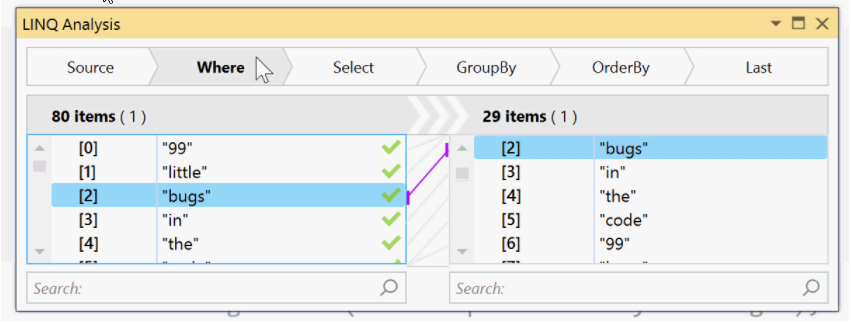
\includegraphics[scale=0.6]{chapter1/img/linq.png}

К сожалению, исходный код OzCode закрыт, расширение работает только с LINQ внутри отладчика Visual Studio, поэтому невозможно понять как он работает. 
